\documentclass[10pt,paper=letter]{scrartcl}
\usepackage[alttitle]{cjquines}

\begin{document}

\title{VCSMS PRIME}
\subtitle{Program for Inducing Mathematical Excellence}
\author{Session 8: Algebraic Manipulation}
\date{October 6, 2017}

\maketitle
\setlength{\unitlength}{1in}
\begin{picture}(0,0)
  \put(5.5,0.5){\hbox{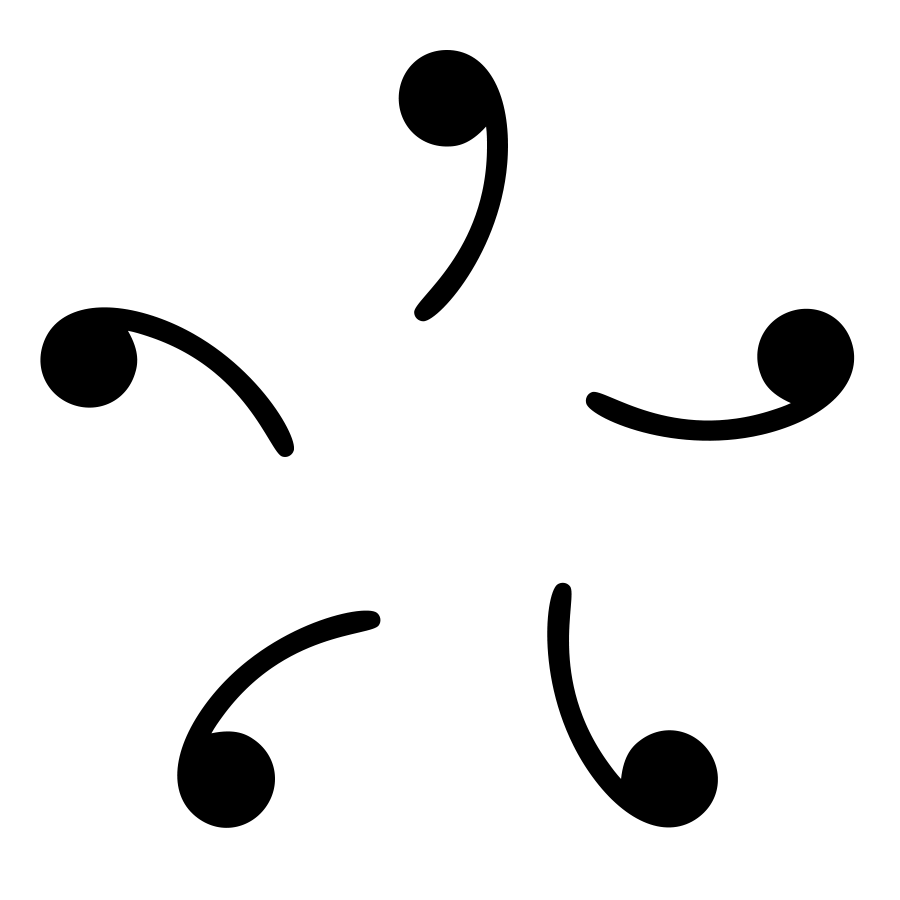
\includegraphics[width=0.9in]{logo.png}}}
\end{picture}
\vspace{-3.5em}

\subsubsection*{Lecture problems}

\begin{enumerate}
  \item (AI14) Define $f: \RR^2 \rightarrow \RR^2$ by $f(x, y) = (2x - y, x + 2y)$. Let $f^0(x, y) = (x, y)$ and, for each $n \in \NN$, $f^n(x, y) = f(f^{n-1}(x, y))$. Determine the distance between $f^{2016}\del{4/5, 3/5}$ and the origin.
  \item Solve the equation $x^4 + (x-2)^4 + 16 = 0$.
  \item Factorize $x^3 + y^3 - 3xy + 1$.
  \item (Sipnayan 2016) Find all $x$ satisfying $\cbrt{20x + \cbrt{20x + \cbrt{20x + 16}}} = 16$.
  \item (AIME 1990/4) Solve $\dfrac1{x^2-10x-29} + \dfrac1{x^2-10x-45} - \dfrac2{x^2-10x-69} = 0$.
  \item Factorize $(x + y - 2z)^3 + (y + z - 2x)^3 + (z + x - 2y)^3$.
  \item (ARML 2016) Factorize $13^4 + 16^5 - 172^2$, given it is the product of three distinct primes.
  \item (AI9) Find the integer which is closest to the value of $\del{\sqrt[6]{5^6 + 1} - \sqrt[6]{5^6 - 1}}^{-1}$.
  \item Given $x^2 - 3x + 1 = 0$, find the value of $x^5 + x^{-5}$.
  \item Solve the equation $x^4 - 6x^3 - 11x^2 - 6x + 1 = 0$.
  \item Prove that the product of four consecutive integers plus one is always a perfect square.
  \item (MMC) Given $6x^2 + 47x + 77 = (2x + 11)(3x + 7)$, factorize $64{,}777$.
  \item Suppose $x + 3y = 3$, $y + 3z = 4$, and $z + 3x = 5$. Find $x$.
  \item (AII1) Let $x$ and $y$ satisfy $\dfrac{x}{x^2y^2 - 1} - \dfrac1{x} = 4$ and $\dfrac{x^2y}{x^2y^2 - 1} + y = 2$. Find all possible values of $xy$.
  \item (AIME 1989/8) Find $16x_1+25x_2+36x_3+49x_4+64x_5+81x_6+100x_7$ given that \begin{align*}x_1+4x_2+9x_3+16x_4+25x_5+36x_6+49x_7&=1\\ 4x_1+9x_2+16x_3+25x_4+36x_5+49x_6+64x_7&=12\\ 9x_1+16x_2+25x_3+36x_4+49x_5+64x_6+81x_7&=123\end{align*}
  \item (AIME 1990/15) Let $f(n) = ax^n + by^n$. Given $f(1) = 3, f(2) = 7, f(3) = 16, f(4) = 42$, find $f(5)$.
  \item (AIME 2014/14) Find all real solutions to $\dfrac3{x-3} + \dfrac5{x-5} + \dfrac{17}{x-17} + \dfrac{19}{x-19} = x^2 - 11x - 4$.
\end{enumerate}

\subsubsection*{Abusing symmetry again}

\begin{itemize}
  \item Algebraic manipulation -- substitution, factorization, manipulation -- usually only has one end goal. To create symmetry. (Almost) all of the problems today deal with this.
\end{itemize}

\newpage

\subsubsection*{Substitution}

\begin{itemize}
  \item Problem 1: Substituting $x, y \to 2x - y, x + 2y$ directly to $\sqrt{x^2 + y^2}$ shows that it's multiplied by $\sqrt{5}$ each time. The symmetry arises when the terms in $(2x - y)^2$ and $(x + 2y)^2$ cancel.
  \item Problem 2: We force symmetry by substituting $x \to y + 1$. The terms in $(y + 1)^2$ and $(y - 1)^2$ cancel.
  \item Problem 3: Exchanging any two variables keeps the expression the same, which means it's \emph{symmetric}. When dealing with symmetric expressions, we usually try substituting $x+y, xy \to a, b$, because of the Fundamental Theorem of Symmetric Polynomials. This is $a^3 - 3ab - 3b + 1$, and there's an $a+1$ factor. 
  \item Problem 4: Substitution again. You substitute the whole expression into the $16$ in the innermost infinitely many times, to get $\cbrt{20x + \cbrt{20x + \cdots}} = 16$, which is more symmetric. Then substitute $16$ for the whole expression to get $\cbrt{20x + 16} = 16$.
  \item Problem 5: By letting $x^2 - 10x - 29 \rightarrow a$, and \emph{then} multiplying out, it's much easier.
\end{itemize}

\subsubsection*{Factorization}

\begin{itemize}
  \item Problem 6: There are a few factorizations you are expected to know, and one of them is $a^3 + b^3 + c^3 - 3abc = (a + b + c)(a^2 + b^2 + c^2 - ab - bc - ca)$. But when $a + b + c = 0$, this becomes $a^3 + b^3 + c^3 = 3abc$.
  \item Problem 7: Use Sophie--Germain: $a^4 + 4b^4 = (a^2 + 2ab + 2b^2)(a^2 - 2ab + 2b^2)$. $16^5$ is $2^{20}$ and $13^4 - 172^2$ is $1 - 2^{10}$ via difference of two squares. Multiply both sides by $2^{10} + 1$ and then factor using Sophie--Germain on $1^4 + 4 \cdot \del{2^7}^4$.
  \item Problem 8: Factor $2 = (5^6 + 1) - (5^6 - 1)$ using difference of two squares, then two cubes.
\end{itemize}

\subsubsection*{Manipulation}

\begin{itemize}
  \item Problem 9: Divide both sides by $x$ to get $x + 1/x = 3$. There are several ways to get $x^5 + x^{-5}$. We can take the fifth power and use the smaller powers, or we can recurse more generally by relating $x^n + x^{-n}$ and $x^{n+1} + x^{-(n+1)}$.
  \item Problem 10: Divide both sides by $x^2$ and use the substitution $x + 1/x \rightarrow a$. 
  \item Problem 11: Suppose the smallest was $n$. Then $n(n+1)(n+2)(n+3) + 1$. To make it easier, pair multiply $n(n+3)$ and $(n+1)(n+2)$, then substitute $n^2 + 3n + 2 \rightarrow a$.
  \item Problem 12: Substitute $x = 100$.
  \item Problem 13: Add all the equations and divide by $5$ to find $x + y + z = 12/5$. Subtract from the second to eliminate $y$ and use the third to find $x$.
  \item Problem 14: Force symmetry, multiply the first by $xy$ and subtract from the second. Solve for $y$ in terms of $x$, substitute, simplify.
  \item Problem 15: Remember the method of finite differences? The perfect squares are quadratic, so the second difference is constant. 
  \item Problem 16: We want to relate $f(n)$ and $f(n+1)$. Like we did in Problem 9 for $x^n + x^{-n}$ and $x^{n+1} + x^{-(n+1)}$, we can see $f(n)(x + y) = f(n+1) + xyf(n-1)$.
  \item Problem 17: The key idea is to add $4$ to both sides. The fraction $3/(x-3)$ becomes $x/(x-3)$, etc. Cancel out $x$ and substitue $x \to y+11$ for symmetry. Add opposite terms and cancel out $y$.
\end{itemize}

\end{document}
